\chapter{State of the Art} \label{chap:sota} \minitoc

In this Chapter, we will discuss the most relevant work for the aforementioned problem of detecting data pattern shifts in real-time computations over true sliding windows using resource-lightweight approaches on streaming systems. We present a wide analysis of several categories of algorithms that seemed like viable options to build the desired system.

\section{Detecting Change in Data Streams} \label{sec:change-detect}

For static data sets, it is reasonable to assume that the data was generated by a fixed process, for example, the data is a sample from a static distribution. But a data stream has necessarily a temporal dimension, and the underlying process that generates the data stream can change over time \cite{Aggarwal-Evolving-Data-Streams} \cite{Domingos-Mining-Time-Data-Streams}. It is this change in the underlying distribution that we want to detect and report as a data pattern shift.

\subsection{A two window paradigm algorithm for change detection}
\label{subsec:2-window}

The authors of \cite{Kifer-Detecting-Change} propose an algorithm for change detection in data streams. The only assumption made is that data points are generated independently. The authors propose that detecting change in data streams can be reduced to testing if two windows have different underlying distributions. Thus the change detection algorithm works on a two-window paradigm.

Figure \ref{fig:change-detection-2-windows} contains the pseudocode presented by the authors. The proposed method uses two windows, a reference \textit{W\textsubscript{1}} and a sliding one \textit{W\textsubscript{2}}. The authors used tuple-based windows of size \textit{k} and the sliding window was a true sliding one, as described in Section \ref{sec:windows}. The reference window \textit{W\textsubscript{2}} works as a \textit{baseline} and contains the first \textit{k} points of the stream that occurred after the last detected change.

The algorithm begins by filling both windows with the first \textit{k} tuples. Then it slides window \textit{W\textsubscript{2}} (by one, since it is a true sliding window). It does this \textit{k} times. In between slides, the algorithm checks for change by applying the \textit{d} function, which measures the discrepancy between the two windows contents, \textit{W\textsubscript{1}} and \textit{W\textsubscript{2}}. Whenever this discrepancy is above a certain threshold $\alpha$, the algorithm reports a change in the data stream. Then it repeats the whole process, re-initializing both windows with the next \textit{k} items and proceeding as already described. 

\begin{figure}[!htb]
    \begin{center}
      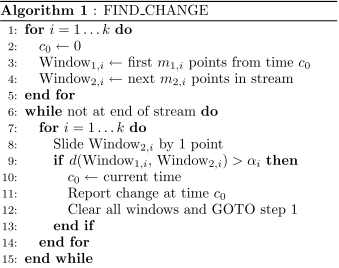
\includegraphics[scale=0.8]{figures/2-windows-change-pseudocode.png}
      \caption{Two window method for data stream change detection}
      \label{fig:change-detection-2-windows}
    \end{center}
\end{figure}

This algorithm reduces change detection in data streams to testing whether two samples, the \textit{reference} and the \textit{sliding window} contents, are generated by different distributions. Consequently, the authors study the case of detecting differences in distribution between two samples. This is the purpose of the \textit{d} function. The authors evaluate many statistical tests as possible implementations of this \textit{d} function that must truly quantify an intuitive notion of change. 

Experiments were made using the following statistical tests as the \textit{d} function: Wilcoxon signed-rank, $\phi$\textsubscript{A} and $\Xi$\textsubscript{A}. The Wilcoxon test is well known but the $\phi$\textsubscript{A} and the $\Xi$\textsubscript{A} statistical tests were defined by the authors. Since computing these three statistical tests for our windows contents takes identical time and space, we consider that a thorough analysis of each one is out of scope for this Thesis, as it does not provide relevant information. 

The authors conclude that no test is best in all of the experiments done. However, the $\phi$\textsubscript{A} and $\Xi$\textsubscript{A} statistics vastly outperformed the others in some tests and did not perform that much worse in other test cases.

Diving deeper in the algorithm presented in \ref{fig:change-detection-2-windows} we now analyze the computation of the \textit{d} function value. In the authors' work, efficient computation of the previously mentioned statistical tests --- \textit{i.e.} the value of function \textit{d} --- is further explored and an algorithm for such is presented. First, the \textit{KS structure} is presented. The formal definition given by the authors is shown in Figure \ref{fig:ks-structure}


\begin{figure}[!htb]
    \begin{center}
      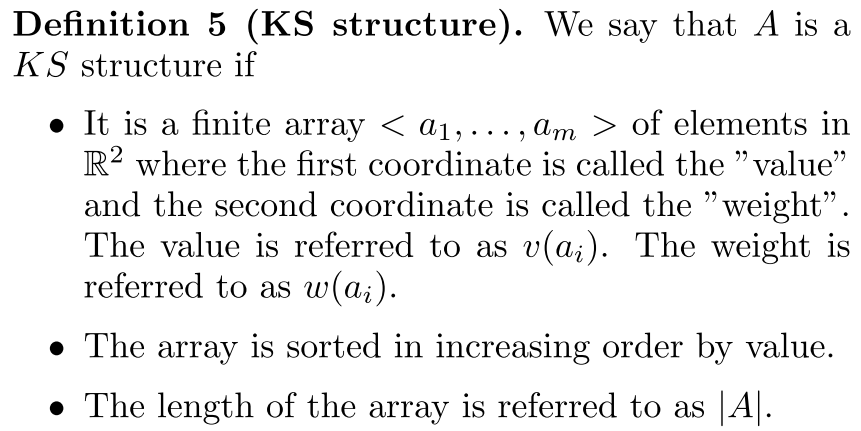
\includegraphics[scale=0.4]{figures/ks-structure.png}
      \caption{Formal definition of the KS structure}
      \label{fig:ks-structure}
    \end{center}
\end{figure}

The KS structure is built from the reference \textit{W\textsubscript{1}} and sliding \textit{W\textsubscript{2}} windows. Consider the pair \textit{(\textit{W\textsubscript{1}}, \textit{W\textsubscript{2}})} where the size of both windows is \textit{k}. Creating the KS structure \textit{Z} of size \textit{2k} is done by joining the elements from \textit{W\textsubscript{1}} and \textit{W\textsubscript{2}}. As stated in \ref{fig:ks-structure}, each element of \textit{Z} will have a value and a weight. The values will be the actual elements joined. The weights of elements coming from \textit{W\textsubscript{1}} will be \textit{-1/k} while the weights of elements coming from \textit{W\textsubscript{2}} will be \textit{1/k}. The final KS structure \textit{Z} must be sorted in increasing order by value. The KS structure \textit{Z} can be maintained throughout running time by making use of a balanced tree, such as a B-tree, in \textit{O(log(2k))} time. By making use of the KS structure, all of the mentioned statistics can be computed in \textit{O(2k)} time. 

\subsubsection{Time complexity analysis}
%k to initialize and when change is detected
%k * d
%d 
 %nlog(2k) to initialize tree and when change is detected
 %log(2k) to maintain the tree
The algorithm begins by collecting the first \textit{k} tuples. Both windows will have size \textit{k}. This takes \textit{O(k)} time but is a task that will only occur on initialization and on change detection, upon which the window contents must reset, as described in \ref{fig:change-detection-2-windows}. For each of the next \textit{k} iterations the function \textit{d} will be computed and compared to the threshold $\alpha$. As previously mentioned, computing the value of \textit{d} can be done in \textit{O(log(2k))} time per iteration. However, the initial time cost of initializing the balanced tree is of \textit{O(k log(2k))}. 

Initialization is not frequent. It occurs once at the beginning of execution and once per change detection upon which the algorithm resets the windows' contents. To provide an accurate time complexity, we take into account the probability \textit{P} of change occurring and being detected leading to a reset. Assuming \textit{P} is within $[0, 1]$, we have a time complexity of \textit{O(P(k + k log(2k)))} per reset --- \textit{i.e.} the probability of a reset occurring times \textit{O(k)} to initialize the windows' contents plus \textit{O(k log(2k))} to build the balanced tree.

In runtime, the algorithm will perform \textit{k} iterations where it computes the \textit{d} function value, taking \textit{O(log(2k))} per iteration, amounting to a time complexity of \textit{O(k log(2k)}.

Putting both initialization and runtime complexities we have a total time complexity of \textit{O(P(k + k log(2k)) + k log(2k))}.

\subsubsection{Space complexity analysis}

The algorithm presented makes use of two \textit{k} sized windows and one balanced tree of size \textit{k} as well. This represents a space complexity of \textit{O(k+k+k)} or \textit{O(3k)}.

\subsubsection{Applicability to our Hypothesis}

The algorithm for change detection presented in Subsection \ref{subsec:2-window} has time complexity of \textit{O(P(k + k log(2k)) + k log(2k))}. and space complexity of \textit{O(3k)}, with \textit{k} as a window size constant. 

In this Thesis, we want to detect and alert data pattern shifts so detecting change in data streams is directly applicable to our use case. However, our focus is on a lightweight solution and this algorithm has a linear space complexity, so it does not fit our scope as a possible solution.

\section{Pattern Mining}

Taking on a new approach, in this Section, we explore pattern mining algorithms rather than algorithms that detect change in data streams. The idea behind using pattern mining algorithms being that if we can maintain a list of frequent patterns we would be able to detect when said patterns change --- \textit{i.e.} the list changes. Change in the frequent mined patterns would be associated with a data pattern shift and immediately reported. 

\subsection{Mining Frequent Patterns: the FP-Stream structure}

The authors of \cite{Giannella-Mining-Frequent-Patterns} developed a data structure named \textit{FP-Stream} --- that summarizes frequent data patterns -- and algorithms to build and incrementally maintain it.

We agree with the author's statement that it is \textit{"unrealistic to hold all streaming data in the limited main memory"}. With this in mind, they divide patterns into three categories: frequent, sub-frequent and infrequent patterns. The focus of their work is the mining and maintenance of frequent and sub-frequent patterns since the latter might become frequent later. Thus, infrequent patterns are discarded, using less memory.

The FP-Stream structure consists of a frequent pattern tree (FP-Tree \cite{Han-FP-tree}) with tilted-time windows in each of the nodes.

The authors are not very explicit on the definition of a tilted-time window. They claim we are \textit{"often interested in recent changes at a fine granularity, but long term changes at a coarse granularity"} and that tilted-time windows fit such use case. Figure \ref{fig:tilted-time-window} shows such a window and was withdrawn from the paper. In it, we see the 4 quarters of the last hour, then the last 24 hours and finally 31 days. They claim that \textit{"one can compute frequent itemsets in the last hour with the precision of quarter of an hour, the last day with the precision of hour, and so on, until the whole month"}.


\begin{figure}[!htb]
    \begin{center}
      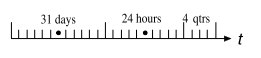
\includegraphics[scale=1]{figures/tilted-time-window.png}
      \caption{Tilted-time window}
      \label{fig:tilted-time-window}
    \end{center}
\end{figure}

An FP-Tree \cite{Han-FP-tree} as shown in Figure \ref{fig:fptree}, is a tree representation of frequent patterns. Each node in the frequent pattern tree represents a pattern and its frequency (\textit{support} column in the Figure), recorded in the node. The same tree construction algorithm from \cite{Han-FP-tree} is used in the FP-Stream algorithm. 

\begin{figure}[!htb]
    \begin{center}
      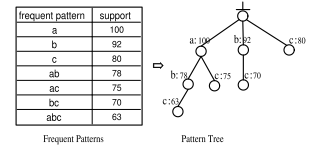
\includegraphics[scale=1]{figures/fptree.png}
      \caption{FP-Tree}
      \label{fig:fptree}
    \end{center}
\end{figure}

The authors propose using only one frequent pattern tree, where at each node, the frequency for each tilted-time window is maintained. Figure \ref{fig:fpstream} shows the FP-Stream structure, as an example of a frequent pattern tree with tilted-time windows embedded in each node.

\begin{figure}[!htb]
    \begin{center}
      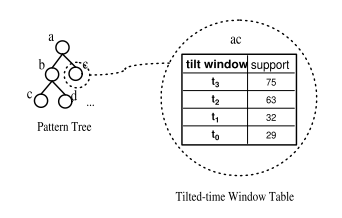
\includegraphics[scale=0.8]{figures/fp-stream.png}
      \caption{FP-Stream}
      \label{fig:fpstream}
    \end{center}
\end{figure}

The algorithm for constructing and maintaining the FP-Stream structure is given as a high-level list of instructions. The algorithm groups incoming streaming data into batches. Initialization is done only when the first batch is complete. As the transactions for the first batch arrived, the frequencies for all items are computed. Once all transactions for the first batch have arrived, the batch is scanned to create an FP-tree structure, pruning all infrequent items -- \textit{i.e.} below a certain frequency threshold. Finally, an FP-Stream structure is created by mining the frequent items from the FP-Tree.

The incremental update of the FP-Stream as data arrives is described on a very high level and does not add relevant information to understand time and space complexity without knowledge of the FP-Tree algorithm, on which it heavily relies. Further research will be done to perform a more thorough analysis of this algorithm, starting with the analysis of \cite{Han-FP-tree}.

\subsubsection{Applicability to our Hypothesis}

No definitive conclusions can be made without the full time and space complexity analysis. However, the maintenance of a frequent pattern tree and tilted-time windows for each of the nodes might reveal to memory intensive, discarding this as a valid solution.

\subsection{Neighbor-Based Pattern Detection for Windows Over Streaming Data: the Extra-N algorithm}

The authors of \cite{Yang-Neighbor-Based-Pattern-Detection} propose a method for incremental detection of neighbor based patterns, namely density-based clusters and distance-based outliers, specifically for sliding windows scenarios. Figure \ref{fig:plot-cluster-outlier} is an example of the previous two mentioned neighbor based patterns. Formal definitions for both distance-based outliers \ref{fig:distance-outlier-def} and density-based clusters \ref{fig:density-cluster-def} are provided.

\begin{figure}[!htb]
    \begin{center}
      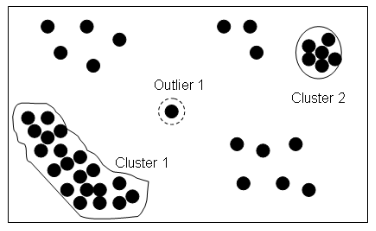
\includegraphics[scale=0.8]{figures/density-distance-based.png}
      \caption[Clustering and outlier identification plot]{Two density-based clusters and one distance-based outlier determined by neighbour-based pattern detection algorithms}
      \label{fig:plot-cluster-outlier}
    \end{center}
\end{figure}

\begin{figure}[!htb]
    \begin{center}
      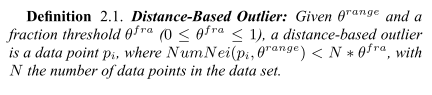
\includegraphics[scale=0.8]{figures/distance-based-outlier-def.png}
      \caption{Formal definition of distance-based outliers}
      \label{fig:distance-outlier-def}
    \end{center}
\end{figure}

\begin{figure}[!htb]
    \begin{center}
      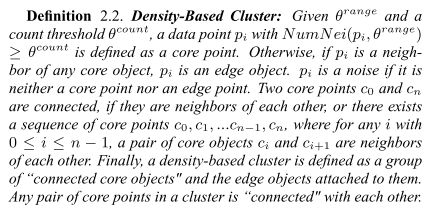
\includegraphics[scale=0.8]{figures/density-based-cluster-def.png}
      \caption{Formal definition of density-based clusters}
      \label{fig:density-cluster-def}
    \end{center}
\end{figure}

Density-based clusters label data points as \textit{core points}, \textit{edge points} or \textit{noise}. These classifications are explained in \ref{fig:density-cluster-def}. Data points are classified based on the number of neighbors they have within a range $\theta\textsuperscript{range}$, measured versus a $\theta\textsuperscript{count}$. In brief, if a data point has more than $\theta\textsuperscript{count}$ neighbors within $\theta\textsuperscript{range}$ it is classified as a \textit{core point}. If it does not but it is a neighbor of a core point, then it is an \textit{edge point}. Otherwise, it is considered \textit{noise}. 

The authors make use of the \textit{“predictability"} property of the expiration of existing objects. In other words, given a window with a fixed slide size, they predetermine the \textit{life-span} of any data point in the window on arrival --- \textit{i.e.} the future windows it will belong to. This leads to the notion of \textit{predicted views}. Given the objects in a current window, they predict the pattern structures that will persist in subsequent windows by considering the objects in the current window and abstract these predicted pattern structures into \textit{“predicted views"} of each future window. This technique allows the efficient maintenance of neighborship counts by pre-handling the eventual expiring effect of new data points.

In the paper, the authors first propose the Abstract-C and Abstract-M algorithms. Ultimately, they combine all the desirable properties of each algorithm into Extra-N. 

\subsubsection{Abstract-C}
Abstract-C was the first proposed algorithm. The main idea is to maintain for each data point \textit{p\textsubscript{i}} the number of neighbors it has rather than the actual list of neighbors. The main advantage of this approach is the reduced memory footprint since only a count is stored --- a single integer --- instead of a list of pointers --- to all neighbors.

When a data point \textit{p\textsubscript{i}} expires, the count of each of \textit{p\textsubscript{i}}'s neighbors must be decremented by one --- since \textit{p\textsubscript{i}} no longer exists. However, we are unable to reach \textit{p\textsubscript{i}}'s neighbors since in Abstract-C only a count of neighbors is stored --- rather than pointers to each of the neighbors.

The solution to this problem is exploiting the previously presented \textit{predictability} property. The key idea is to predict the expiration of any data point \textit{p\textsubscript{i}} and pre-handle the impact it has on \textit{p\textsubscript{i}}'s neighbours. The authors introduce the concept of \textit{"lifetime neighbour counts"} or \textit{lt\_cnt}. The \textit{lt\_cnt} of a data point \textit{p\textsubscript{i}} corresponds to a sequence of \textit{predicted neighbour counts} --- \textit{i.e.} the number of \textit{predicted neighbours} \textit{p\textsubscript{i}} has in any future window where he exists. More precisely, each entry on \textit{pi.lt\_cnt} records the number of \textit{p\textsubscript{i}}'s current neighbours that are known to survive in the corresponding future window. Furthermore, the length of \textit{p\textsubscript{i}.lt\_cnt} is kept equal to \textit{p\textsubscript{i}.lifespan}, decreasing by one after each window slide, removing the left most entry. The authors provide the following example: consider a window \textit{W\textsubscript{i}} and a data point \textit{p\textsubscript{i}} with three neighbours, \textit{p\textsubscript{1}}, \textit{p\textsubscript{2}} and \textit{p\textsubscript{3}}. Applying the \textit{predictability} property makes it possible to compute the lifespan of all points. Assume \textit{p\textsubscript{1}} expires after \textit{W\textsubscript{i}}, \textit{p\textsubscript{2}} and \textit{p\textsubscript{3}} expire after \textit{W\textsubscript{i+1}} and \textit{p\textsubscript{i}} expires after \textit{W\textsubscript{i+2}}. This implies that at \textit{W\textsubscript{i}}, \textit{p\textsubscript{i}.lt\_cnt} = \{\textit{W\textsubscript{i}}: 3, \textit{W\textsubscript{i+1}}: 2, \textit{W\textsubscript{i+2}}: 0\}. 

According to the definition given in \ref{fig:distance-outlier-def}, the lifetime neighbor counts (\textit{lt\_cnt}) carry enough information to compute distance-based outliers: for each data point \textit{p\textsubscript{i}} check if the first (current) element of \textit{p\textsubscript{i}.lt\_cnt} is less than  \textit{$\theta\textsuperscript{fra}$} $\times$ \textit{N} to decide whether a data point is an outlier or not, with \textit{N} as the number of data points. Similarly, the core objects for the density-based clusters can be computed by comparing the first element of \textit{p\textsubscript{i}.lt\_cnt} with \textit{$\theta$\textsuperscript{count}}. However, the \textit{lt\_cnt} array does not carry enough information to generate the density-based clusters. Despite being able  to find all core points in the window, we can not group them into clusters. In order to compute that, Abstract-C analyzes each core point and the surrounding $\theta\textsuperscript{range}$ area in the window to reconstruct the clusters.

In conclusion, Abstract-C achieves linear memory consumption in the number of data points in the window. However, since it reconstructs the clusters for each core object in the window, it has \textit{O(CP)} time complexity, with \textit{CP} as the total number of core points. Hence, its performance largely depends on  \textit{CP}, which can vary from 0 -- no core points --- to the total window size --- all core points. 

\subsubsection{Abstract-M}
Abstract-M is proposed as an Abstract-C enhancement by introducing the notion of \textit{cluster memberships}, achieved by attributing a \textit{clusterID} to each data point.

The main challenge of this approach is discounting the effect of expired data points. The removal of any data point on any cluster may result in the total break of the cluster into multiple smaller ones, which may persist or degrade to noise. Furthermore, when a cluster is split, the newly formed clusters must be attributed with new \textit{clusterID}s --- \textit{i.e.} every single data point in those clusters must be relabeled with the new \textit{clusterID}.

Once again, the solution to handle expiring data points relies on the predictability property. Knowing the data points that exist in each window means we can also know the set of future clusters and points that belong. This is included in the \textit{predicted views} concept previously mentioned. In brief, the \textit{predicted clusters} are created using such predicted views for each of the future windows.

Addition of new data points may cause three changes to the clusters: \textit{birth} of a new cluster, \textit{expansion} of an existing one and \textit{merge} of multiple existing clusters. When adding a new data point, mark it with a new \textit{clusterID} in case of a \textit{birth} or in an \textit{expansion} case mark it with the \textit{clusterID} of the cluster it belongs to. Handling the \textit{merge} of multiple clusters is done by using a tree structure where two or more sibling \textit{clusterID}s are in fact part of a bigger cluster with the \textit{clusterID} stored in their parent. For example, if cluster \textit{ID1} and cluster \textit{ID2} are merged into a new cluster \textit{ID3} by the arrival of a new data point, they are inserted as children of the node containing \textit{ID3}.

New data points may join existing neighborhoods of existing data points and may promote them to core points by making the size of their neighborhood greater or equal to \textit{$\theta$\textsuperscript{count}}. Once such promotion happens, the promoted core point needs to communicate to its neighbors its new role, since noise in its neighborhood becomes edge points and is given a \textit{clusterID}. Since there are no connections from the promoted data point to its neighbors, Abstract-M analyzes each of the promoted core points and the $\theta\textsuperscript{range}$ area around them to find the points requiring state update. 

In conclusion, Abstract-M remains linear in memory regarding the number of window data points. However, since the number of promoted core points tends to be smaller and is always less or equal to the number of core points, this is an improvement on Abstract-C.

\subsubsection{Extra-N}

Abstract-M still performs range queries (area with $\theta\textsuperscript{range}$ diameter) for each of the promoted core points. To improve upon this, Extra-N combines the neighborship maintenance mechanisms proposed in Abstract-C and Abstract-M.

The authors state that different information is required from different classes of data points (\textit{core}, \textit{edge} or \textit{noise}). For example, maintaining a list of points to neighbors is required for a non-core point while neighbor counts are sufficient for core points. More precisely, Extra-N marks each data point \textit{p\textsubscript{i}} with a \textit{clusterID} in all windows where \textit{p\textsubscript{i}} is predicted to be a core point while keeping the exact list of neighbors (pointers) of \textit{p\textsubscript{i}} for all windows where he is predicted to be noise or an edge point. This way, the Extra-N algorithm stores the amount of information needed to compute both distance-based outliers and density-based clusters according to their definitions, \ref{fig:distance-outlier-def} and \ref{fig:density-cluster-def} respectively.

\subsubsection{Time complexity analysis}
Extra-N only performs range queries for incoming data points. This means that for each new data point \textit{p\textsubscript{i}}, Extra-N will search the area of diameter $\theta\textsuperscript{range}$ around it and update on it neighbors. In conclusion, the time complexity of Extra-N is \textit{O(n)} where \textit{n} is the number of new data points. 

\subsubsection{Space complexity analysis}
In summary, Extra-N keeps the memory consumption linear to the number of data points in the window without performing unnecessary range queries.

\subsubsection{Applicability to our Hypothesis}
While a linear complexity fits most of the scenarios, it does not fit ours since we aim to build a low memory footprint solution, ideally with space complexity of \textit{O(1)}. Hence, this algorithm will be of no use to us.


\section{Anomaly Detection}
Anomaly detection refers to the process of finding anomalies in data. An anomaly relates to a point in time where the behavior of the system does not match the expected one. Hence, under this definition, an anomaly does not necessarily imply a problem. 

With the study of anomaly detection algorithms, we intend to search for algorithms that identify data pattern shifts as anomalies. If any of the approaches searched for is not computationally intensive it will be considered valid for the final solution. 

\subsection{Real-Time Stream Anomaly Detection with Hierarchical Temporal Memory}

In \cite{Ahmad-HTM}, the authors present an anomaly detection technique based on an on-line algorithm called Hierarchical Temporal Memory (HTM). HTM has a few properties that are desirable for data stream anomaly detection scenarios. First, it is an unsupervised algorithm that requires no labels. This property comes in handy when monitoring a data stream in real-time, where labels for incoming data will likely be absent. Additionally, HTM adapts to noisy domains. In other words, random variations in the underlying distribution of incoming data that do not persist throughout time will be ignored. Furthermore, HTM detects both spatial and temporal anomalies --- \textit{i.e.} changes in magnitudes of data or unusual timing for particular patterns, respectively.   

HTM is also an online learning algorithm, meaning that it adapts to changing statistics of the underlying data stream. In other words, if there is a sudden random increase in a specific data point attribute, the algorithm will produce an alert. However, if that initially thought to be a random spike becomes frequent then the algorithm adapts and assimilates this as "a new reality". Hence, it stops classifying it as an anomaly. Unfortunately, this property is not desirable in our system. Our stream monitoring system must report changes relatively to an initial static configuration and should not accept a new distribution as the new standard.

\subsubsection{Applicability to our Hypothesis}
Online learning algorithms that adapt to data pattern shifts and eventually consider them regular patterns are not viable methods to accomplish our goal of building a monitoring system that alerts data pattern shifts continuously until they match the initial configuration again. Additionally, insights produced by machine learning models are not human-understandable, rendering the user unable to understand why an anomaly report was made. In conclusion, we do not deem HTM applicable to our solution.

\subsection{DeepAnT}

DeepAnT \cite{Munir-DeepAnT} is a deep learning-based approach for the detection of anomalies in time series data, that uses unlabeled data to capture and learn the data distribution of the stream used to forecast the normal behavior of the time series data. It is unsupervised - \textit{i.e.} it requires no labels - which is an advantage in a data streaming scenario where real-time decisions have to be made before labels are effectively-known. It is capable of detecting point anomalies in time series data with periodic and seasonal characteristics.

DeepAnT employs a Convolutional Neural Network (CNN) as its \textit{time series predictor} module. Before monitoring a data stream, the CNN must be trained. The model can be trained with a small data set while achieving good generalization capabilities due to the effective parameter sharing of the CNN. Additionally, the data set used to train the model thus not require labels and may up to 5\% of the data set may correspond to anomalous data.

\subsubsection{Applicability to our Hypothesis}

Similar to the HTM algorithm presented, DeepAnT adapts to the underlying distribution of the data stream. In other words, if the data patterns shift from the initial configuration but stabilize, DeepAnT will accept it as it is. As mentioned, our goal is to build a monitoring system that alerts data pattern shifts continuously, until they match the initial configuration again. Furthermore, DeepAnT uses deep learning which is actually a subset of machine learning and just as inexplicable. In summary, we do not deem DeepAnT usable for our use case.

\iffalse

\section{Sliding Window Aggregations}
Aggregations and Sliding Window Aggregations (SWAGs) have been introduced in Section \ref{sec:aggregations}. In this Section, we analyze algorithms that allow for sliding window aggregations utilizing a set of different aggregation operators. In other words, different algorithms work with different aggregation categories based on their properties. The properties of different categories of aggregations were defined in Section \ref{sec:aggregations} and summarized in Table \ref{tbl:operations-properties}.

\subsection{DABA}
\subsubsection{Time complexity analysis}
\subsubsection{Space complexity analysis}
\subsubsection{Applicability to our Hypothesis}

\fi

\section{Probabilistic Data Structures} \label{sec:pds}
Probabilistic data structures use hash functions to compactly represent a set of items while approximately answering queries with fixed error bounds. This way, these structures are capable of processing huge volumes of data. They require a single pass through the data, which is appropriate for a streaming scenario. Probabilistic data structures have constant space and time complexity \cite{Singh-PDS-BIGD} making them candidate methods to build our real-time and low memory footprint system.

\subsection{Membership Queries and the Bloom Filter}
A Bloom filter \cite{BLOOM-BLOOMFILTER} is a probabilistic data structure that allows membership queries on a set of elements. Bloom filters answer the query: "Is element \textit{el} in the set of seen elements so far?". Being a probabilistic data structure, Bloom filters do not always give a certain answer. \textit{False positive} matches are possible --- \textit{i.e.} saying \textit{el} is in the set when it is not --- but \textit{false negatives} are not --- \textit{i.e.} saying \textit{el} is not in the set but it actually is. In other words, a bloom filter will accurately identify all items that do not belong in the set but will misclassify some items as being present in the set. Hence, a query returns either \textit{possibly in set} or \textit{definitely not in set}. 

A Bloom filter is an array of bits of size \textit{m}. A Bloom Filter makes use of \textit{k} hash functions. The choice of the \textit{m} and \textit{k} constants will determine the false positive rate. 

Initially, all bits are set to 0. Adding an element is done by determining which positions should be set to 1. To that end, the new element is fed into each hash function that maps the element to an array position. The resultant \textit{k} outputs are used as the \textit{k} positions of the array to be set to 1.

Performing a membership query --- \textit{i.e.} testing if an element \textit{el} is in the set --- is done by feeding \textit{el} into each one of the \textit{k} hash functions in order to get an array of positions. If \textit{el} was already in the set then all \textit{k} positions should be 1. If any position contains a 0 then the element is \textit{definitely not in set}, as shown in Figure \ref{fig:bloom-filter} from \cite{bloom-filter-wikipedia}. If all positions are 1 then the element is \textit{possibly in the set}. 

The reason a Bloom Filter does not provide 100\% certainty that \textit{el} is in the set in case of all positions being 1 is that hash functions may give the same position for two different elements. For example, hash functions \textit{k\textsubscript{1}}, \textit{k\textsubscript{2}} and \textit{k\textsubscript{3}} may map an element \textit{el1} to positions $[1,2,3]$ and an element \textit{el2} to positions $[4,5,6]$. This way, bits in positions $[1,2,3,4,5,6]$ are set to 1. Given a new element \textit{el3} not yet seen, hash functions \textit{k\textsubscript{1}}, \textit{k\textsubscript{2}} and \textit{k\textsubscript{3}} may map it to $[1,3,5]$ and all of these positions are already 1 because of the previous elements. Thus the Bloom filter returns \textit{"possibly in set"} because all bits are set to 1 when in reality \textit{el3} was not in the set. This is considered a \textit{false positive}.


\begin{figure}[!htb]
    \begin{center}
      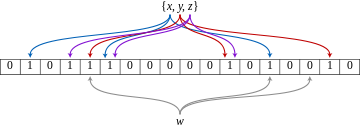
\includegraphics[scale=0.8]{figures/bloom-filter.png}
      \caption[Bloom filter membership test]{Bloom filter membership test of element 'W'. Finding one '0' indicates that it is not in the set.}
      \label{fig:bloom-filter}
    \end{center}
\end{figure}


An improvement to this structure was defined in \cite{Kirsch-Better-Bloom} where the authors attempt to reduce the overhead of bloom filters operations such as adding a new element or answering a query by focusing on the hash functions. The proposed method is based on hashing literature. It has been shown that multiple hash functions can be created from the combination of only two hash functions. This means that a new hash function \textit{g} can be produced based on  two other independent and uniform existing hash functions, \textit{h1} and \textit{h2}. The new hash function will map elements to a universe ranging from \textit{0} to \textit{p-1} and will be defined as \textit{$g(x) = h1(x) + ih2(x) mod p$}. Since the only nontrivial computations performed by a Bloom filter are the evaluations of pseudo-random hash functions, any reduction in the required number of pseudo-random hash functions yields a reduction in the time required to add an element or query a Bloom filter.

Bloom filters are not the only approximate aggregators that use hash functions as a basis of their algorithm. All of the studied probabilistic data structures do so. Therefore, the technique proposed is beneficial in HyperLogLogs, Count-Min Sketches and Bloom filters.

\subsubsection{Time complexity analysis}
Considering a Bloom filter with \textit{m} bits and \textit{k} hash functions, insertion and search will both take \textit{O(k)} time because all there is to do is run the input through all of the \textit{k} hash functions and set the bits in the given positions to 1. Note the time complexity does not at all depend on the number of elements in it and that \textit{k} will be a rather small constant (magnitude of $10^1$). Hence, the Bloom filter is said to have constant time complexity (\textit{O(1)}).

\subsubsection{Space complexity analysis}
Considering a Bloom filter with \textit{m} bits, the space required is simply the array of \textit{m} bits, thus \textit{O(m)} space complexity. Similarly to the time complexity analysis, we point out that \textit{m} will be constant and that each of the array elements occupies 1 bit. Thus the Bloom filter has a constant space complexity (\textit{O(1)}).

\subsubsection{Applicability to our Hypothesis}
Bloom filters exhibit constant space and time complexity making it great methods to test our hypothesis. Their false positive rate is tolerable in most scenarios and can be controlled by tweaking the values of \textit{m} and \textit{k}.

\subsection{Item Frequency and the Count-Min Sketch}

A Count–Min Sketch (CMS) is a probabilistic data structure that gives an estimate of the frequency of each element in the data set. The estimate is a minimum count. The real frequency of an element will never be lower than the given estimate, hence the name \textit{count min}. The CMS is first introduced in \cite{Cormode-CMS}. 

A CMS is represented by a two-dimensional array (or matrix) with width \textit{w} and depth \textit{d}. A CMS will make use of \textit{d} hash functions --- \textit{i.e.} each associated with one row of the matrix. Each hash function will map elements to a position between 1 and \textit{w} --- \textit{i.e.} the column of the two-dimensional array.

Initially, all of the matrix positions are 0. When adding an element, for each row \textit{i} of the \textit{d} rows in the matrix, hash the element using that row's hash function to obtain \textit{j}. Lastly, for all obtained pairs of \textit{i} and \textit{j}, increment matrix cells \textit{(i, j)} value by 1, as seen in Figure \ref{fig:cms}.

\begin{figure}[!htb]
    \begin{center}
      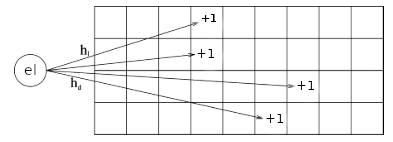
\includegraphics[scale=0.8]{figures/cms.png}
      \caption[Count-Min Sketch update]{CMS mapping element \textit{el} using \textit{d} hash functions to determine the column position for each row and increment it}
      \label{fig:cms}
    \end{center}
\end{figure}

Retrieving the minimum frequency of an element \textit{el} can be done by taking the minimum value of all row counts for \textit{el}. Mathematically, the frequency estimate is given by
\[ min \{matrix[i][\textit{h\textsubscript{i}}(el)]\} \]
for each row \textit{i} of the total \textit{d} rows.    

%The CMS is not always correct because...

\subsubsection{Time complexity analysis}
When adding an element or querying the frequency of one, the Count-Min Sketch loops through each row and applies a constant in time hash function, proceeding to a position update or retrieval, respectively. Hence, the time complexity is of \textit{O(d)}. Given \textit{d} is a constant, the CMS has constant time complexity --- \textit{O(1)}.

\subsubsection{Space complexity analysis}
The Count-Min Sketch relies on a two-dimensional matrix as its only data structure. The memory used will correspond to the \textit{wd} counts, hence \textit{O(wd)} space complexity. Since both \textit{w} and \textit{d} are constants, the CMS has constant space complexity --- \textit{O(1)}.

\subsubsection{Applicability to our Hypothesis}
Count-Min Sketches are constant in both time and space. Similarly to Bloom filters, this makes them ideal candidates for our solution. 

\subsection{Cardinality Estimation and the HyperLogLog}
In the paper \cite{Flajolet-PCA}, a class of probabilistic counting algorithms is introduced to estimate the number of distinct elements based on \textit{"bit pattern observables"} in the binary representation of the hashed values --- \textit{i.e.} patterns related to the number and positions of 0's and 1's in a binary string.

\subsubsection{LogLog}
Later on, the same authors propose the LogLog algorithm \cite{Flajolet-LogLog}. In LogLog, the \textit{bit pattern observable} recorded from each item's hash value is the position of the leftmost 1-bit. The authors claim it is related to the total number of distinct elements in the data set.

\subsubsection{HyperLogLog}
A couple of years later, the same authors propose HyperLogLog (HLL) in \cite{Flajolet-HLL}. HLL solves the problem of counting distinct elements in a data set, also known as the cardinality of the data set \cite{Flajolet-HLL}. HLL gives an approximation of the cardinality of the data set. 

In HyperLogLog, an item is hashed into a binary string. Based on the first \textit{n} bits, the string is passed on to one of the \textit{$2^n$ buckets}. After discarding the first \textit{n} bits, the number of trailing 0's plus 1 is counted. In other words, the position of the leftmost 1-bit is recorded, like in LogLog. This is what is stored in each bucket: the maximum value of the position of the leftmost 1-bit of all seen items so far. 

%TODO \textbf{HYPERLOGLOG HOW IT WORKS IMAGE}

Finally, the estimate for the number of distinct elements will be $2^p$, where \textit{p} is the harmonic mean of all bucket values holding the maximum leftmost 1-bit position value. This computation of a harmonic mean over \textit{m} buckets is called stochastic averaging and is the main difference between HyperLogLog and LogLog. Given the nature of streaming systems, it is also important to notice that this algorithm is suitable for a distributed system since each of the buckets can be updated independently.

\subsubsection{Time complexity analysis}
Adding an item is tantamount to hashing it, determining the corresponding bucket based on the first \textit{n} bits, count the leftmost 1-bit position and update the bucket value if need be. Estimating the cardinality of the set amounts to finding the maximum value \textit{p} between all buckets and computing $2^p$. Hence, both inserting a new element and estimating the cardinality take constant time --- \textit{O(1)}.

\subsubsection{Space complexity analysis}
Quoting Flajolet et al. about the memory consumption and error in the approximations obtained in their experiments in  \cite{Flajolet-HLL}: 
\say{cardinalities till values over N = $10^9$ can be estimated with a typical accuracy of 2\% using 1.5kB (kilobyte) of storage.}

HyperLogLog uses \textit{m} buckets that store a single integer value. This gives it complexity of \textit{O(m)} where \textit{m} is a small constant. Hence, HyperLogLog has constant space complexity --- \textit{O(1)}.

\subsubsection{Applicability to our Hypothesis}
Similar to the previously studied probabilistic data structures, HyperLogLog (HLL) has constant space and time complexity while giving an approximation of a set's cardinality. Hence, HLLs are considered valuable methods for our work.


\iffalse

\section{Sliding Window Aggregation with Probabilistic Data Structures}
In Section \ref{sec:pds} we presented a set of probabilistic data structures constant in time and space complexity. These structures aggregate an endless stream of data. However, when working under a sliding window context there is the need not only to insert new events but to evict old ones. Probabilistic data structures aggregate all incoming data but have no way of removing elements. 

In this Section, we explore and analyze sliding window implementations of the previously discussed probabilistic data structures.

\subsection{Sliding HyperLogLog}
HyperLogLog  (HLL) will only be useful in our system if it can be implemented efficiently in a sliding window fashion. That is precisely what \cite{Chabchoub-Sliding-HLL} presents us with. In this paper, the original HLL algorithm from \cite{Flajolet-HLL} is adapted to a sliding window scenario with the use of slightly more memory. More importantly, the estimate is as accurate as in the original HLL algorithm. 

It consumes additional space compared to the original algorithm of at most $5\textit{m}ln(\textit{n}/\textit{m})$ bytes, with \textit{m} being the number of buckets and \textit{n} the number of distinct elements actually flowing through the stream. As explained by the authors, storing additional context is required so that the algorithm can work in a sliding window fashion. Thus they propose maintaining a shortlist of packets. A packet consists of a pair \textit{(ti, Ri)}, where the \textit{ti} is the arrival time of the packet and \textit{Ri} is the position of the leftmost 1-bit in the binary representation of the hashed value associated with that packet. The idea is to store only packets that are a possible maximum over a future window. Hence, this list is called \textit{List of Future Possible Maxima (LFPM)}. Furthermore, they propose efficient methods for the insertion and eviction of new and old elements from the window, respectively. In this sliding version, one LFPM is kept per bucket. For that reason, estimating the set cardinality is similar to the original HyperLogLog: compute the harmonic mean for all buckets. The value of each bucket is the highest \textit{Ri} for that bucket. Hence, the extra required memory in the Sliding HyperLogLog algorithm presented is given by the size of the \textit{m} lists of future possible maxima.

\subsubsection{Time complexity analysis}

\subsubsection{Space complexity analysis}

\subsubsection{Applicability to our Hypothesis}

\fi

%\textbf{image for sliding hyperloglog}
 